\chapter{Installing SCAS}
\label{chap_installation}

The SCAS source files along with installation scripts can be downloaded from our public GIT repository \url{https://github.com/vipinkmenon/fpgadriver}.
The source file contains both the hardware as well as software components for SCAS.
The hardware components include all the source files for creating the FPGA configuration in verilog format, the Xilinx IP cores in synthesised (netlist) format, the constraints file for directing the FPGA place and route tools and some scripts for enabling command line execution of Xilinx development tools.
The software components mainly include the source file for the FPGA driver, the user library and a number of example applications.
The hardware development can be done on both Windows as well as Linux operating systems, but the SCAS FPGA driver is only supported on Ubuntu platform.

\begin{figure}[h]
\centering
\includegraphics[width=7cm]{figures/inst_hierarchy.pdf}
\caption{Directory Structure}
\label{inst_hierarchy}
\end{figure}

\noindent The hierarchy of SCAS components are shown in Fig.~\ref{inst_hierarchy} and described in Table~\ref{tab:hierarchy}.
The user library contains all the APIs required by the user application software to communicate with the hardware.
A single installation script is provided, which will install the Linux driver, user libraries and the ''hardware'' components.
To install the required file, switch the working directory into \emph{fpgadriver/install} and run the following commands.\\

\hspace*{4.45cm}{\texttt{chmod 777 install.sh}}\\
\hspace*{5cm}{\texttt{sudo ./install}}\\

Running script builds the driver and the user library. 
It then installs the driver and copies the user library (libfpga.so) to the shared user library location (/usr/lib/).
The installation also copies the hardware source files to a global location (/usr/include/fpga), so that the user application can access these components from any location similar to accessing the software shared library.
Once the installation is finished, the user software application can include the \emph{fpga.h} user library header file to use the driver APIs and can use \emph{-lfpga} as the library path during compiling.

\input \TBLDIR/hierarchy.tex

Use the example bitstream provided (v6\_top.bit or v7\_top.bit depending upon the target FPGA board) in the fpga/bitstream directory to program the FPGA for verification.
If you find difficulty in installing the Xilinx USB-JTAG cable for Ubuntu, follow the instructions at \url{http://www.george-smart.co.uk/wiki/Xilinx_JTAG_Linux#Newer_UDEV_.28Ubuntu_9.10.29}.
Reboot the host system since this is the first installation and the host needs to detect the board.
Now make sure that hardware is properly detected.
If you can visually inspect the board after rebooting, there should be 3 LEDs glowing and 1 LED constantly blinking.
\begin{itemize}
\item{LED0 : Blinking. Indicating Proper PCIe clock}
\item{LED1 : Internal PLL lock for DRAM}
\item{LED2 : PCIe link status}
\item{LED3 : DRAM link status}
\end{itemize}
It has been observed that ML605 board intermittently fails to detect DRAM.
In this case, power cycle the FPGA board, reprogram the FPGA and reboot.
To make sure that the host system has properly detected the FPGA board, execute the following command in the terminal\\
\hspace*{4.45cm}{\texttt{sudo lspci -vvv -d 10EE:*}}\\\\
lspci command lists the PCIe devices in the system and 0x10EE is the vendor ID for Xilinx.
This command will give detailed information about the configuration space of the FPGA PCIe endpoint.
The capability register values should indicate the device is Gen.2 capable and the link width is x4.
The control register indicates what is the configuration set by the host for the FPGA device.
For low-end host systems, the host may configure the device as only Gen.1 capable or in the worst-case as Gen.1 capable with only x1 link width.
This can severely affect the system performance.
If you have spare PCIe slots, try to plug-in the board to a different slot if this scenario occurs.

Make sure that the lspci command lists ''fpga'' as the driver for the endpoint device.
If the host fails to detect the driver, use the ''dmesg'' command to detect possible errors.\\\\
\hspace*{4.45cm}{\texttt{dmesg | grep fpga}}\\\\
If the hardware and driver installations are successful, go the application directory.
Run the \emph{fpga\_pio} example application by executing\\\\
\hspace*{4.45cm}{\texttt{./fpga\_pio}}\\\\
This should return the FPGA hardware version and the system health parameters.
The health parameter values are valid only on ML605 board since the VC707 board lacks the on-board sensors to measure these values.

Detailed description of integrating user applications and writing the application software are given in Chapters \ref{chap_integration} and \ref{chap_software}.